\newcommand\SubProbIN{\Objective_{in}}
\newcommand\SubProbOUT{\Objective_{out}}
\newcommand\SubProbUP{\Objective_{up}}
\newcommand\SubProbDOWN{\Objective_{down}}

%%%%%%%%%%%%%%%%%%%%%%%%%%%%%%%%%%%%%%%%%%%%%%%%%%%%%%%%%%%%%%%%%%%%%%
\section{Introduction}

In this chapter we solve the optimization problem \eqnref{opt-scene},
which asks for the maximizer $\OptimalScene$ of
\begin{equation}
  \Objective(\Scene) =
    \sum_{j=1}^{\Width} \PixelPayoff(j,\seam_j,\WallOrient_j) -
    \sum_{i=0}^{\NumWalls-1} \CornerPenalty(i;\Scene) ~,
\end{equation}
where
\begin{equation}
  \Scene =
  ( x_1,y_1,\WallOrient_1,
   ~x_2,y_2,\WallOrient_2,
   ~\ldots,
   ~x_{n-1},y_{n-1},\WallOrient_{n-1}, ~x_n )
\end{equation}
is an indoor Manhattan scene in vertex representation.

We assume that the scene rotation $\SceneR$ as well as the floor and
ceiling position $\Zs$ have been recovered as discussed in
\chapref{orientation}. We further assume that all images are rectified
as in \eqnref{rectification}. The algorithms presented in this section
are valid without the rectification step, but assuming rectification
considerably simplifies their presentation.

Our solution uses dynamic programming to efficiently solve the
maximization \eqnref{opt-scene}. We develop the algorithm conceptually
before formalising it.

We wish to constrain hypotheses to those representing valid indoor
Manhattan models. In terms of individual pixels this introduces
complicated dependencies between large groups of pixels, since
assigning a particular label to any one pixel restricts which labels
can be assigned to other pixels in the same column. We therefore cast
the minimisation directly in terms of the vertex representation
introduced in chapter 4.

We have already seen that every indoor Manhattan scene can be
represented as a left--to--right sequence of wall segments, and every
image column intersects exactly one wall segment. A direct result is
that the placement of each wall is conditionally independent of the
other walls given its left and right neighbours. For example,
\figref{partial-model} shows a partial model as well as several wall
segments that could be appended to it. Some of the candidates are
feasible (green dashes) and some are not (red dashes); however, note
that once the wall segment from $c_3$ to $c_4$ is fixed, the choices
for walls following $c_4$ are independent of choices made for wall
segments prior to $c_3$. Later we will formalize and prove this
statement; for now we proceed conceptually.

We are led to a decomposition of the problem into a series of
sub--problems of the form ``find the minimum--cost \textit{partial}
model spanning columns $0 \ldots x$'' for various $x$. To solve this
we enumerate over all possible walls $\Wall$ that terminate at $x$,
then for each we recursively solve sub--problems corresponding to the
left extent of the wall. This recursion terminates at the left
boundary of the image since each recursion leads to an $x'$ that is
strictly less than $x$. As in all dynamic programming, the solution to
each sub--problem is cached to avoid redundant computation, then a
simple counting argument shows that the algorithm has polynomial
complexity.

The authors have experienced some difficulty giving a clear and
concise description of the algorithm in past publications. We proceed
therefore with a short intuitive discussion before presenting our
algorithm formally.

%%%%%%%%%%%%%%%%%%%%%%%%%%%%%%%%%%%%%%%%%%%%%%%%%%%%%%%%%%%%%%%%%%%%%%
\section{Intuition}

Consider a path finding problem in which we must are asked to identify
the path from left to right through a cost matrix that minimizes the
sum of costs along the path. An example cost matrix and the
least--cost path is shown in \figref{seam-carving}. The solution to
this simple problem is a special case of Dijkstra's algorithm and is
well known in the literature, but for pedagogical purposes we describe
it here.

One view of the solution --- slightly non--standard but relevant to
the algorithm to come --- is as a series of sub--problems as
follows. Let $h(\Pixel)$ be the sub--problem: ``what is the minimum
energy path from any point on the left edge of the matrix to
$\Pixel$?'' Then we say that any a path $\vect{Y}$ \textit{satisfies}
$h(\Pixel)$ if the last entry in $\vect{Y}$ equals $\Pixel$, and that
$\vect{Y}$ \textit{solves} $h(\Pixel)$ if, in addition, $\vect{Y}$ has
minimal cost among all such paths.

These definitions are useful because we can solve each sub--problem in
terms of other sub--problems, all the way down to a trivial boundary
condition,
\begin{equation}
  \label{eq:seam-carving}
  h(x,y) = 
  \begin{cases}
    \min \Bigl(
      h(x-1,y-1),
      h(x-1,y),
      h(x-1,y+1)
    \Bigr) + c(x,y),
    & \mbox{if } x>0 \\
    0 & \mbox{if } x=0
  \end{cases}
\end{equation}
where $c$ is the cost matrix. The algorithm corresponding to
\eqnref{seam-carving} is simply a recursive function of $(x,y)$ that
evaluates \eqnref{seam-carving}, then the least--cost path is
recovered by back--tracking afterwards.

The optimization problem that is the subject of this chapter can be
thought of as a path--finding problem where the seam representation
constitutes a path from left--to--right through the image, and the
payoff function constitutes a cost matrix. Unfortunately, however, the
penalty term has no counterpart in the above framework, so
\eqnref{opt-scene} cannot be solved using recurrence relations of the
form \eqnref{seam-carving}. This is because the framework above has no
regularization term to penalize complicated paths over those
comprising simple straight edges.

\subsection{Viterbi Decoding}
Let us generalize \eqnref{seam-carving} by removing the continuity
constraint on paths and introducing a penalty for transitions. Let the
cost of transitioning from $(x,y)$ to $(x+1,z)$ be $a(y,z)$. Then the
cost of a path $\vect{Y}$ is
\begin{equation}
  \label{eq:viterbi-cost}
  \sum_{i=1}^n c(i,Y_i) - a(Y_i,Y_{i+1})
\end{equation}
and the corresponding recurrence relation is
\begin{equation}
  \label{eq:viterbi-recurrence}
  h(x,y) = 
  \begin{cases}
    \min_{1\leq z\leq m}\limits h(x-1,z) - a(z,y),& \mbox{if } x>0\\
    0,& \mbox{if } x=0 ~.
  \end{cases}
\end{equation}
If the cost and transition matrices correspond to log--likelihoods
then this is precisely the Viterbi algorithm for maximum--likelihood
inference in hidden Markov models.

Unfortunately, we are still unable to express the penalty term
$\ScenePenalty(\Scene)$ in a framework such as
\eqnref{viterbi-recurrence} because $\ScenePenalty$ introduces a bias
for solutions that consists of a few straight edges, but there is no
notion of ``straightness'' in \eqnref{seam-carving}. Indeed the
problem is worsened considerably because we seek a path that
corresponds to some 3D reconstruction, but many paths will not
correspond to any physically realisable reconstruction.

\subsection{The Diagonal Route Model}

Model where paths can go straight or along either of two diagonals.

The recurrence relation looks like
\begin{equation}
  h(x,y,a) = \max \Bigl[ h(x-1,y+a,a), 
    \max_{a'}\limits \bigl( h(x-1, ya-', a'), T(a',a) \bigr) \Bigl]
\end{equation}

We have managed to express a prior on the number of straight
sub--segments in a dynamic programming formulation.

There's a lot further to go yet, but the final model will look
something like the above.

%%%%%%%%%%%%%%%%%%%%%%%%%%%%%%%%%%%%%%%%%%%%%%%%%%%%%%%%%%%%%%%%%%%%%%
\section{Preliminaries}
\label{sect:preliminaries}

\subsection{Definitions}

\subsubsection{Partial Scenes}

We begin by generalizing the notion of a scene to a partial scene,
which spans the portion of the image from its left edge to some image
column $x$, $0 \leq x \leq W$. An example of a partial scene in shown
in \figref{partial-scene}.

\begin{figure}[tb]
  \centering
  \label{fig:partial-scene}
  \includegraphics[width=0.29\textwidth]{partial-model}
  \caption{A partial model terminating at column $c_4$ with several
    feasible (green dashed) and infeasible (red dashed) wall
    segments.}
\end{figure}

\begin{definition}
  \label{def:scene-len}
  The length of a scene $\Scene$ in vertex representation
  \eqnref{vertex-repr} is the number of distinct walls in $\Scene$ and
  is denoted $\Length{\Scene}$.
\end{definition}

\begin{definition}
  \label{def:partial-scene}
  A partial scene $\PartialScene$ is a scene with
  $x_{\Length{\Scene}}<\Width$. The corresponding seam representation
  is
  \begin{equation}
    \PartialSeam = \{(\seam_j,\WallOrient_j)\}_{j=0}^{\Length{\PartialScene}}
  \end{equation}
  where the values $\seam_j,\WallOrient_j$ are defined as for ordinary
  seams by equation \eqnref{seam-from-scene}.
\end{definition}

We now define two operations for manipulating walls. Walls are
represented by the 4--tuple $(x_a,y_a,\WallOrient,x_b)$ as defined by
equation \eqnref{wall-def}.

\begin{definition}
  The termination point of a wall $\Wall$ is the triple
  $(x_b,y_b,\WallOrient)$ where $(x_b,y_b)$ is the location of the
  lower--right corner of $\Wall$ as defined by equation \eqnref{qi}.

  We say that a scene $\Scene$ terminates at $(x_b,y_b,\WallOrient)$
  if its right--most wall terminates at $(x_b,y_b,\WallOrient)$. We will
  also say that a scene terminates at column $x_b$ if it terminates at
  $(x_b,y_b,\WallOrient)$ for some $y_b,\WallOrient$.
\end{definition}

\begin{definition}
  \label{def:truncation}
  The $q$--truncation of the partial scene $\PartialScene$ is scene obtained
  by removing the last $q$ walls from $\PartialScene$,
  \begin{equation}
    \PartialScene_{-q} = 
    ( x_1,y_1,\WallOrient_1,
    \ldots,
    ~x_{\SceneLen-q-1},y_{\SceneLen-q-1},\WallOrient_{\SceneLen-q-1},
    ~x_{\SceneLen-q} )~.
  \end{equation}
\end{definition}

\begin{definition}
  \label{def:concatentation}
  The concatentation of the scene $\PartialScene$ with the wall
  $\Wall=(x_a,y,\WallOrient,x_b)$ is defined if and only if
  $\PartialScene$ terminates at column $x_a$ and equals
  \begin{equation}
    \PartialScene \concat \Wall = 
    ( x_1,y_1,\WallOrient_1,
    \ldots,
    ~x_{\SceneLen-1},y_{\SceneLen-1},\WallOrient_{\SceneLen-1},
    ~x_a, y, \WallOrient, ~ x_b )
  \end{equation}
\end{definition}

\subsubsection{Additive Scores}

Here we introduce notions of scores for walls and scenes. Our
definitions broadly mirror the definition for full scenes in equation
\eqnref{scene-payoff}; however, there is in general no direct
probabilistic interpretation for the definitions below. This poses no
difficulty to the probabilistic consistency of our algorith since in
this setting we are simply solving the optimization problem
\eqnref{opt-scene}. If $\PixelPayoff$ has been configured to represent
the log--likelihood of some probabilistic model then the solution we
find will correspond to MAP inference, but we are not concerned with
the internals of the probabilistic model in this chapter.

\begin{definition}
  \label{def:scene-score}
  The score obtained by a partial scene $\PartialScene$ that
  terminates at column $x_b$ under the payoff function $\ScenePayoff$
  is
  \begin{equation}
    \Objective(\PartialScene) = \sum_{j=0}^{x_b} 
      \PixelPayoff(j,\seam_j,\WallOrient_j) - 
      \sum_{i=0}^{\SceneLen} \CornerPenalty(i;\PartialScene)
  \end{equation}
\end{definition}

\begin{definition}
  \label{def:wall-score}
  The payoff for a wall $\Wall=(x_a,y,\WallOrient,x_b)$ under the
  payoff function $\ScenePayoff$ is
  \begin{equation}
    \WallPayoff(\Wall) = \sum_{j=x_a}^{x_b-1}
      \PixelPayoff(j,\seam_j,\WallOrient_j) ~.
  \end{equation}
\end{definition}

We note the following additivity property of scores.

\begin{lemma}
  \label{lemma:additive-scores}
  Let $\Scene$ be a scene and $\Wall$ be a wall and suppose
  $\Scene\concat\Wall$ is well--defined. Then the score obtained by
  $\Scene\concat\Wall$ is
  \begin{equation}
    \Objective(\Scene\concat\Wall) = 
      \Objective(\Scene) + \WallPayoff(\Wall) - 
      \CornerPenalty(\Scene,\Wall)
  \end{equation}
  where $\CornerPenalty(\Scene,\Wall)$ is the penalty
  for the corner added to the scene as a result of appending $\Wall$.
\end{lemma}
\begin{proof}
  Follows directly from definitions \ref{def:scene-score} and
  \ref{def:wall-score}.
\end{proof}

\subsubsection{Feasibility}

Not all scenes permitted by the vertex representation are physically
realisable since some would imply the existence of infinitely thin
walls. Figure XXX shows three examples of impossible scenes. Lee \etal
\cite{Lee09} showed that physical realisability can be deduced from
simple tests on the ordering of walls and the relative positions of
vanishing points. Although we do not wish to repeat their work here,
several decomposability properties of the physical realisability tests
are central to the validity of the dynamic programming algorithm to be
presented, so we re--state them here

\begin{definition}
  \label{def:feasible-corners}
  The $i$\th corner of the scene $\Scene$ is feasible if and only if
  it passes the tests described in \cite{Lee09}, which is
  functionally dependent on the values
  \begin{equation}
    y_b,~\WallOrient_i,~x_{i+1},~y_{i+1},~\WallOrient_{i+1}
  \end{equation}
  where the $i$\th wall in $\Scene$ terminates at
  $(x_{i+1},y_b,\WallOrient_i)$.
\end{definition}

\begin{lemma}
  \label{def:feasible-scenes}
  $\Scene$ is feasible if and only if all corners in $\Scene$ are feasible.
\end{lemma}
\begin{proof}
  See \cite{Lee09}
\end{proof}

\begin{lemma}
  \label{lemma:trunc-feasibility}
  Let $\Scene$ be a feasible scene. Then any truncation $\Scene_{-q}$ is
  feasible.
\end{lemma}
\begin{proof}
  Any truncation $\Scene_{-q}$ consists of a subset of the corners in
  $\Scene$, all of which are feasible by assumption.
\end{proof}

\begin{lemma}
  \label{lemma:concat-feasibility}
  Let $\Wall=(x_b,y_b,\WallOrient_b,x_c)$ be a wall and let $\Scene$ and
  $\OtherScene$ be feasible scenes terminating at
  $(x_b,y_a,\WallOrient_a)$. Then $\Scene\concat\Wall$ is feasible if
  and only if $\OtherScene\concat\Wall$ is feasible.
\end{lemma}
\begin{proof}
  Suppose $\Scene\concat\Wall$ is feasible. Then we need to show that
  each corner in $\OtherScene\concat\Wall$ is feasible. By assumption
  the first $\Length{\OtherScene}$ corners are feasible. According to
  definition \ref{def:feasible-corners}, the feasibility of the last corner
  is a function of the values
  \begin{equation}
    y_a,~\WallOrient_a,~x_b,~y_b,~\WallOrient_b,
  \end{equation}
  But these values are identical to the last corner in
  $\Scene\concat\Wall$, which is feasible by assumption, so
  $\OtherScene\concat\Wall$ is feasible. The opposite
  direction of implication is obtained by a symmetric argument.
\end{proof}

%%%%%%%%%%%%%%%%%%%%%%%%%%%%%%%%%%%%%%%%%%%%%%%%%%%%%%%%%%%%%%%%%%%%%%
\section{Proposed Algorithm}

We now present the sub--problems and the recurrence relations
comprising the first version of our solution to \eqnref{opt-scene}.

\begin{definition}
  \label{def:sub-problem-in}
  A scene $\Scene$ satisfies the sub--problem $\SubProbIN(x,y,a)$ if
  $\Scene$ is feasible and $\Scene$ terminates at $(x,y,a)$.

  A scene $\Scene$ solves the sub--problem $\SubProbIN(x,y,a)$ if it
  satisfies $\SubProbIN(x,y,a)$ and there is no other scene satisfying
  $\SubProbIN(x,y,a)$ that obtains a greater score.
\end{definition}

\Figref{fin-examples} shows three examples of different scenes
satisfying a particular sub--problem.

\begin{figure}[tb]
  \centering
  \includegraphics[width=0.75\textwidth]{fin-hypotheses}
  \caption{Three models satisfying the sub--problem
    $\SubProbIN(x,y,a)$.}
  \label{fig:fin-examples}
\end{figure}

\begin{lemma}
  \label{lemma:solutions-exist}
  There is a solution to $\SubProbIN(x,y,\WallOrient)$ for all $1 \leq x \leq W$,
  $1 \leq y \leq H$, $\WallOrient\in\{1,2\}$.
\end{lemma}
\begin{proof}
  Simply construct a scene $\Scene$ with a sequence of alternating
  concave/convex corners in the interval $[1,x]$. Non--occluding
  corners are always feasible \cite{Lee09}, so $\Scene$ satisfies
  $\SubProbIN(x,y,\WallOrient)$. There are finitely many scenes and at
  least one satisfies $\SubProbIN(x,y,\WallOrient)$; therefore
  $\SubProbIN(x,y,\WallOrient)$ has a solution.
\end{proof}

We now turn to the central theorem of this chapter.

\begin{theorem}
  \label{thm:substructure}
  Let $\Scene$ be a scene terminating at $(x,y,\WallOrient)$. Let
  $\TruncScene$ be the 1--truncation of $\Scene$ and let
  $(x',y',\WallOrient')$ be the terminating state of
  $\TruncScene$. If $\Scene$ solves $\SubProbIN(x,y,\WallOrient)$
  then $\TruncScene$ solves $\SubProbIN(x',y,'\WallOrient')$.
\end{theorem}
\begin{proof}
  First note that $\TruncScene$ satisfies
  $\SubProbIN(x',y',\WallOrient')$ since it terminates at
  $(x',y',\WallOrient')$ and is feasibile by Lemma
  \ref{lemma:trunc-feasibility}.

  We show that $\TruncScene$ solves $\SubProbIN(x',y',\WallOrient')$
  by appeal to \textit{reductio}. If $\TruncScene$ does not solve
  $\SubProbIN(x',y',\WallOrient')$ then there exists a scene
  $\CfTruncScene$ satisfying $\SubProbIN(x',y',\WallOrient')$ such
  that
  \begin{equation}
    \label{eq:cf-score}
    \Objective(\CfTruncScene) > \Objective(\TruncScene) ~.
  \end{equation}
  Let $\Wall$ be the right--most wall in $\Scene$ and let $\CfScene =
  \CfTruncScene \concat \Wall$. We have that $\CfScene$ satisfies
  $\SubProbIN(x,y,\WallOrient)$ due to the following:
  \begin{enumerate}
    \item{$\CfScene$ terminates at $(x,y,\WallOrient)$ because its
      right--most wall is $\Wall$, which terminates at
      $(x,y,\WallOrient)$ by assumption.}
    \item{$\CfScene$ is feasible by Lemma
      \ref{lemma:concat-feasibility}.}
  \end{enumerate}
  Next we use Lemma \ref{lemma:additive-scores} to expand the scores
  obtained by $\Scene$ and $\CfScene$,
  \begin{equation}
  \begin{split}
    \label{eq:concat-scores}
    \Objective(\Scene) &=
      \Objective(\TruncScene) + \WallPayoff(\Wall) - 
      \CornerPenalty(\TruncScene,\Wall) \\
    \Objective(\CfScene) &=
      \Objective(\CfTruncScene) + \WallPayoff(\Wall) - 
      \CornerPenalty(\CfTruncScene;\Wall)
  \end{split}
  \end{equation}
  But by an analogous argument to the proof of Lemma
  \ref{lemma:concat-feasibility}, the corner produced by appending
  $\Wall$ to $\TruncScene$ is the same as that produced by appending
  $\Wall$ to $\CfTruncScene$ since $\TruncScene$ and $\CfTruncScene$
  terminating at the same state. Therefore
  \begin{equation}
    \label{eq:equal-penalties}
    \CornerPenalty(\TruncScene,\Wall) =
    \CornerPenalty(\CfTruncScene,\Wall) ~.
  \end{equation}
  Combining \eqnref{cf-score}, \eqnref{concat-scores}, and
  \eqnref{equal-penalties}, we have
  \begin{equation}
    \Objective(\CfScene) > \Objective(\Scene) ~,
  \end{equation}
  but this contradicts the assumption of $\Scene$ as a solution to
  $\SubProbIN(x,y,\WallOrient)$.
\end{proof}

Theorem \ref{thm:substructure} is the main result in the construction
of the dynamic programming solution to \eqnref{opt-scene}. Our first
recurrence relation is provided by corollary
\ref{cor:first-recurrence} below, but first we need to define the
feasible set,
\begin{definition}
  A state $\State$ is a tuple $(x,y,\WallOrient)$. The state space
  $\StateSpace$ is the set of all states,
  \begin{equation}
    \StateSpace = [1,\Width] \cross [1,\Height] \cross \{1,2\} ~.
  \end{equation}
  The feasible set $\FeasibleSet(\State) \subset \StateSpace$ for
  $\State$ is the set of states $\State'$ such that the scene
  \begin{equation}
    \Scene = \Scene' \concat \Wall
  \end{equation}
  is feasible, where $\Scene'$ is any feasible model terminating at
  $\State'$ and $\Wall=(x',y',a,x)$.
\end{definition}

Intuitively one can think of the feasible set as the set of states
``reachable in one step'' from $\State$.

\begin{corollary}
  \label{cor:first-recurrence}
  Let $\State=(x,y,\WallOrient)\in\StateSpace$ be a state with
  $x>1$. Then
  \begin{equation}
    \label{eq:first-recurrence}
    \SubProbIN(\State) = 
    \max_{\State'\in\FeasibleSet(\State)}\limits
    \Bigl( 
      \SubProbIN(\State') + \WallPayoff(\Wall) - \CornerPenalty(\State',\Wall)
    \Bigr) ~,
  \end{equation}
  where
  \begin{equation}
    \label{eq:wall-def}
    \Wall=(x',y',\WallOrient,x) ~.
  \end{equation}
  Further,
  \begin{equation}
    \label{eq:first-boundary}
    \SubProbIN(1,y,\WallOrient) = 0 \quad\quad \forall y,\WallOrient ~.
  \end{equation}
\end{corollary}
\begin{proof}
  Let $\Scene$ be a solution to $\SubProbIN(\State)$. We first show
  that the left side of \eqnref{first-recurrence} is greater than or
  equal to the right side. We then show that the inequality is an
  equality.

  The inequality is established as follows. Let $\Scene'$ be a
  solution to $\SubProbIN(\State')$ for
  $\State'\in\FeasibleSet(\State)$. Let $\Wall$ be as defined in
  \eqnref{wall-def}. We have that
  \begin{enumerate}
    \item{$\Scene'\concat\Wall$ is feasible by the definition of the
      feasible set; and}
    \item{$\Scene'\concat\Wall$ terminates at $\State$ by the definition
      of $\Wall$.}
  \end{enumerate}
  So $\Scene'\concat\Wall$ satisfies $\SubProbIN(\State)$. By the
  assumption of $\Scene$ as the solution to $\SubProbIN(\State)$ we
  therefore have
  \begin{eqnarray}
    \Objective(\Scene)
      &\geq&
    \Objective(\Scene'\concat\Wall)\\
      &\geq&
    \Objective(\Scene') + \WallPayoff(\Wall) -
    \CornerPenalty(\State',\Wall)\\
    \SubProbIN(\State)
      &\geq&
    \SubProbIN(\State') + \WallPayoff(\Wall) -
    \CornerPenalty(\State',\Wall) ~,
  \end{eqnarray}
  thus giving the desired inequality.

  The equality is obtained by noting that theorem
  \ref{thm:substructure} guarantees that there is at least one state
  $\State^*\in\FeasibleSet(\State)$ such that a solution to
  $\SubProbIN(\State^*)$ concatenated with $\Wall$ is a solution to
  $\SubProbIN(\State)$.

  Finally, the boundary condition \eqnref{first-boundary} follows from
  the fact that a scene that terminates at column $1$ does not span
  any part of the image.
\end{proof}

Finally, the cost of the solution to \eqnref{opt-scene} is
\begin{equation}
  \label{eq:opt-entry-point}
  \Objective(\OptimalScene) = 
  \max_{y,\WallOrient} \SubProbIN(\Width,y,\WallOrient) ~.
\end{equation}

We compute $\Objective(\Scene^*)$ by recursively evaluating
$\SubProbIN$ according to \eqnref{first-recurrence} until we reach the
boundary condition \eqnref{first-boundary}. To avoid redundant
computation we cache the result of each evaluation together with the
state $\State'$ corresponding to the maximising term in
\eqnref{first-recurrence}. This allows the desired model
$\OptimalScene$ to be reconstructed by back--tracking once all
evaluations are complete. This is formalised in
\algref{first-solution}.

\begin{algorithm}
  \newcommand\ProcSolve{Solve}
  \newcommand\Cache{{\tt cache}}
  \newcommand\Ptr{{\tt ptrs}}
  \label{alg:scene-to-recon}
  \begin{algorithmic}
    \REQUIRE{$\ScenePayoff$ is a payoff funtion}
    \REQUIRE{$\CornerPenalty$ is a penalty funtion}
    \ENSURE{$\Scene^*$ is the solution to \eqnref{opt-scene}}
    \STATE{$\mbox{\Cache} = \emptyset$}
    \STATE{$\mbox{\Ptr} = \emptyset$}
    \STATE{$\Objective^* = -\infty$}
    \FOR{$y=1$ to $H$}
      \FOR{$\WallOrient \in \{1,2\}$}
        \STATE{$\Objective_{cur} \leftarrow\mbox{\ProcSolve}(W,y,\WallOrient)$}
        \IF{$\Objective_{cur}>\Objective^*$}
          \STATE{$\Objective^* \leftarrow \Objective_{cur}$}
          \STATE{$\State^* \leftarrow \{W,y,\WallOrient\}$}
        \ENDIF
      \ENDFOR
    \ENDFOR
    \STATE{$\Scene^* \leftarrow (W)$}
    \WHILE{$\State^* \neq \emptyset$}
      \STATE{$\Scene^* \leftarrow
        (\State^*_x,\State^*_y,\State^*_{\WallOrient}) \concat
        \Scene^*$}
      \STATE{$\State^* \leftarrow \mbox{\Ptr}(\Scene^*)$}
    \ENDWHILE
  \end{algorithmic}

  \vspace{4mm}\hrule\vspace{1mm}
  \textbf{Subprocedure} \ProcSolve:
  \vspace{1mm}\hrule\vspace{2mm}
  \begin{algorithmic}
    \REQUIRE{$\State=(x,y,\WallOrient)\in\StateSpace$}
    \ENSURE{$\mbox{\Cache}[\State]=\SubProbIN(\State)$}
    \IF{$\State\notin\mbox{\Cache}$}
      \IF{$x = 0$}
        \STATE{$\mbox{\Cache}[\State] \leftarrow 0$}
        \STATE{$\mbox{\Ptr}[\State] \leftarrow \emptyset$}
      \ELSE
        \FORALL{$\State' \in \FeasibleSet(\State)$}
          \STATE{$\Wall\leftarrow(\State_x',\State_y,\State_{\WallOrient},\State_y)$}
          \STATE{$\Objective_{cur} \leftarrow
            \mbox{\ProcSolve}(\State') 
            + \WallPayoff(\Wall) 
            - \CornerPenalty(\State',\Wall)$}
          \IF{$\Objective_{cur}>\mbox{\Cache}[\State]$}
            \STATE{$\mbox{\Cache}[\State] \leftarrow \Objective_{cur}$}
            \STATE{$\mbox{\Ptr}[\State] \leftarrow \State'$}
          \ENDIF
        \ENDFOR
      \ENDIF
    \ENDIF
    \RETURN{$\mbox{\Cache}[\State]$}
  \end{algorithmic}

  \caption{Solve \eqnref{opt-scene} [version 1]}
\end{algorithm}

TODO: expand on how back--tracking is done

\subsubsection{Algorithmic Complexity}
Due to the caching scheme, \eqnref{first-recurrence} is evaluated
at most once for each unique state. There are $2WH$ possible
parameters and the complexity of each evaluation is $O(W^2H)$, since
the minimisation in \eqnref{first-recurrence} is over $O(WH)$
terms and computing each marginal payoff $\ScenePayoff(\Wall)$
requires $O(W)$ additions. The overall complexity of the algorithm
above is therefore $O(W^3H^2K) = O(L^5K)$ where $L=\max(W,H)$.

\subsection{First Refinement: Auxiliary Sub--problems}

The basic algorithm described thus far involves minimising over all
pixels to the left of $\State$ for each state $\State$. In the
previous section we enforced feasibility by explicitly testing each
$\State'$ and omitting any that lead to an infeasible model. In this
section we show that by introducing auxiliary sub--problems we can
deal with feasibility constraints while avoiding the minimization over
$O(L^2)$ items at each evaluation. We introduce three new
sub--problems as follows.
\begin{definition}
  \label{def:aux-sub-problems}
  Let $\Scene$ be a scene terminating at $(x_b,y_b,\WallOrient_b)$ and
  let $\State=(x,y,\WallOrient)$ be a state. Then
  \begin{itemize}
    \item{$\Scene$ satisfies $\SubProbUP(\State)$ iff $\Scene$
      is feasible and $x_b=x$ and $\WallOrient_b=\WallOrient$ and $y_b \leq y$;}
    \item{$\Scene$ satisfies $\SubProbDOWN(\State)$ iff
      $\Scene$ is feasible and $x_b=x$ and $\WallOrient_b=\WallOrient$ and $y_b \geq y$;}
    \item{$\Scene$ satisfies $\SubProbOUT(\State)$ iff
      $\Scene$ is feasible and $x_b=x$ and $\Scene\concat(x,y,\WallOrient,x+1)$ is
      feasible.}
  \end{itemize}
  We say that a scene solves a sub--problem if no other satisfying
  scene obtains greater score.
\end{definition}

Intuitively, the scenes satisfying $\SubProbUP$ and $\SubProbDOWN$ are
those that termate directly above $(x,y)$ and directly below $(x,y)$,
respective. The scenes that satisfy $\SubProbOUT$ are those to which a
wall with lower--left corner $(x,y)$ and orientation $\WallOrient$
could feasibly be added. Figure TODO shows examples of scene
satisfying each of thes above sub--problems.

The purpose of introducing auxiliary sub--problems is to permit a
series of more efficient recurrent relations. We begin with
$\SubProbUP$ and $\SubProbDOWN$.

\begin{corollary}
  Let $\State=(x,y,\WallOrient)\in\StateSpace$ be a state. Then
  \begin{eqnarray}
    \label{eq:fup-recurrence}
    \SubProbUP(x,y,\WallOrient) &=& 
    \begin{cases}
      \max \Bigl(\SubProbIN(x,y,a),
                 \SubProbUP(x,y-1,\WallOrient) \Bigr), &
      \mbox{if } y > 1 \\
      \SubProbIN(x,y,a), & \mbox{if } y=1
    \end{cases}\\
    \label{eq:fdown-recurrence}
    \SubProbDOWN(x,y,\WallOrient) &=& 
    \begin{cases}
      \max \Bigl(\SubProbIN(x,y,\WallOrient),
                 \SubProbDOWN(x,y+1,\WallOrient) \Bigr), &
      \mbox{if } y < H \\
      \SubProbIN(x,y,\WallOrient), & \mbox{if } y=H
    \end{cases}
  \end{eqnarray}
\end{corollary}
\begin{proof}
  We prove \eqnref{fup-recurrence} only; the proof of
  \eqnref{fdown-recurrence} is nearly identical.

  Let $\Scene$ be a solution to $\SubProbUP(x,y,\WallOrient)$ and let
  its terminating state be $(x_b,y_b,\WallOrient_b)$. Consider first
  the case that $y=1$. By the definition of $\SubProbUP$ it must be
  that $\Scene$ terminates at $(x,y,a)$, in which case the
  conditions on $\Scene$ now exactly match those for $\SubProbIN$
  given in definition \ref{def:sub-problem-in}.

  Now suppose $y>1$. Then either $y_b=y$ or $y_b \leq y-1$, with the
  former corresponding again to the sub--problem $\SubProbIN(x,y,a)$
  and the latter to the sub--problem $\SubProbUP(x,y-1,a)$. Therefore,
  we may simply maximise over those two cases.
\end{proof}  

Next we prove recurrence relations for $\SubProbOUT$.

\begin{corollary}
  Let $\State=(x,y,\WallOrient)\in\StateSpace$ be a state. Then
  TODO: deal with feasibility here
  TODO: introduce notation for corner categories properly
  \begin{equation}
    \begin{split}
      \label{eq:fout-recurrence}
      \SubProbOUT(x,y,\WallOrient) = 
      \max_{\WallOrient'\in\{l,r\}} \max \Bigl(
        &\SubProbUP(x,y-1,\WallOrient')
        - \CornerPenalty(x,\WallOrient',\WallOrient,-1),\\
        &\SubProbIN(x,y,\WallOrient')
        - \CornerPenalty(x,\WallOrient',\WallOrient,0),\\
        &\SubProbDOWN(x,y+1,\WallOrient')
        - \CornerPenalty(x,\WallOrient',\WallOrient,+1),
      \Bigr)
    \end{split}
  \end{equation}
\end{corollary}
\begin{proof}
  TODO
\end{proof}

And finally we re--write \eqnref{first-recurrence} in terms of the new
sub--problems as follows.

\begin{corollary}
  \label{cor:fin-recurrence-second}
  Let $\State=(x,y,\WallOrient)\in\StateSpace$ be a state with
  $x>1$. Let $Y_{\State}(x')$ be the intersection of column $x'$ with
  the line through $\vpt_{\WallOrient}$ and $(x,y)$ (see figure
  TODO). Then
  \begin{equation}
    \label{eq:fin-recurrence-second}
    \SubProbIN(x,y,\WallOrient) =
    \max_{x'<x}\limits
    \Bigl(
      \SubProbOUT(x',Y_{\State}(x'),\WallOrient) + \WallPayoff(\Wall)
    \Bigr) ~,
  \end{equation}
  where $\State'=(x,Y_{\State}(x'),\WallOrient)$ and
  $\Wall=(x',Y_{\State}(x'),\WallOrient,x)$ is a wall.
\end{corollary}
\begin{proof}
  TODO
\end{proof}

The dependencies between the sub--problems are illustrated as an
evaluation graph in \figref{eval-graph}.

TODO: mention how this is all implemented.

\subsubsection{Algorithmic Complexity}

By introducing auxiliary sub--problems we have increased the total
number of sub--problems by a factor of 4. However, the sub--problems
$\SubProbUP, \SubProbDOWN,$ and $\SubProbOUT$ have $O(1)$ complexity
and the maximization \eqnref{fin-recurrence-second} is now over $O(L)$
terms (whereas \eqnref{first-recurrence} consists of $O(L^2)$
terms). The complexity of the algorithm in this section is therefore
$O(L^3)$.

\begin{figure}[tb]%
  \centering
  \label{fig:graph-simple}
  \includegraphics[width=0.225\textwidth]{simple-graph}
  \caption{The evaluation graph for a $3 \times 3$ image under
    the naive algorithm.}
\end{figure}

\begin{figure}[tb]%
  \centering
  \label{fig:graph-aux}
  \includegraphics[width=0.49\textwidth]{auxiliary-node-graph}
  \caption{The evaluation graph for a $3 \times 3$ image introducing
    auxiliary sub--problems.}
\end{figure}

\begin{figure}[tb]%
  \centering
  \label{fig:kinked-wall}
  \includegraphics[width=0.2\textwidth]{kinked-wall}
  \caption{The bend introduced by rounding $y'$ to $\hat{y}=\lfloor
    y'+0.5 \rfloor$.}
\end{figure}

\begin{figure}
  \centering
  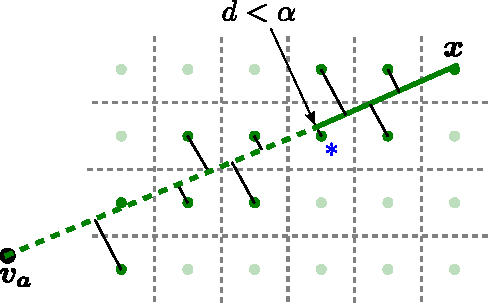
\includegraphics[width=0.35\textwidth]{pixel-residuals}
  \label{fig:pixel-residuals}
  \caption{A line from $\vect{x}$ to
    $\vect{v_a}$ with the distances $d$ to nearby pixel centres (green
    dots). The starred pixel is the first that satisfies
    $d<\epsilon$.}
\end{figure}

\begin{figure}
  \centering
  \includegraphics[width=0.35\textwidth]{eval-graph}
  \label{fig:eval-graph}
  \caption{A graph in which each node represents a
    sub--problem and each edge is a dependence relation. Two columns
    are expanded; other column are omitted for brevity. The green quad
    is a wall corresponding to a particular pair of nodes in the
    graph.}
\end{figure}

\subsection{Second Refinement: From $O(L^3)$ to $O(L^2)$}
Evaluating \eqnref{fin-recurrence-second} remains an $O(W)$ operation
due to the minimisation over $x'$. In this section we to reduce this
to $O(1)$.

Consider recurrence relation \eqnref{fin-recurrence-second}. The
maximization is over columns $x-1,x-2,\ldots,1$. Suppose we split this
set at some column $z$, producing two sets, $Z_+=\{x-1,x-2,\ldots,z\}$
and $Z_-=\{z-1,z-2,\ldots,1\}$. Then the maximizing scene at column
$x$ could be written
\begin{equation}
  \label{eq:fin-split}
  \begin{split}
    \SubProbIN(x,y,\WallOrient) =
    \max\Bigl\{
      &\max_{\State'\in Z_+}\limits \bigl(~
        \SubProbOUT(\State',\WallOrient)
        + \WallPayoff(\Wall) - \CornerPenalty(\State',\Wall)~
      \bigr),\\
      &\max_{\State'\in Z_-}\limits \bigl(~
        \SubProbOUT(\State',\WallOrient)
        + \WallPayoff(\Wall) - \CornerPenalty(\State',\Wall)~
      \bigr)
    \Bigr\} ~.
  \end{split}
\end{equation}
Now compare the maximization over $Z_-$ in \eqnref{fin-split} with the
sub--problem $\SubProbIN(z,\tilde{y},o)$, where $\tilde{y}$ equals
$Y_{\State}(z)$ rounded to the nearest integer. Both maximizations are
over columns $z-1 \ldots 1$. The only difference is that in
\eqnref{fin-split} the $y$--coordinates at each column are
$Y_{\State}(x)$ whereas in $\SubProbIN(z,\tilde{y},o)$ they are
$Y_{\OtherState}(x)$ where $\OtherState=(z,\tilde{y},o)$. If we accept
the latter as an approximation of the former then we could set $z=x-1$
and replace the $O(W)$ maximization over $Z_-$ with a single call to
$\SubProbIN(z,\tilde{y},\WallOrient)$, giving an $O(1)$ expression for
$\SubProbIN$. Unfortunately this is a approximation because the
quantities $Y_{\State}(x)$ and $Y_{\OtherState}(x)$ may differ
substantially, as illustrated in figure TODO. Furthermore, repeatedly
making this approximation in recursive evaluations of $\SubProbIN$
compounds the errors, as illustrated in figure TODO.

\textbf{Alternative Description}

Consider the sub--problem $\SubProbIN(x,y,\WallOrient)$ as formulated
in \eqnref{fin-recurrence-second}. Evaluating $\SubProbIN$ is like
walking along each column $x-1,x-2,...,1$ and considering two
possibilities at each step: insert a corner or continue walking. The
former corresponds to evaluating $\SubProbOUT(x',y',\WallOrient)$; the
latter to $\SubProbIN(x',y',\WallOrient)$. But $y'$ is computed by
intersecting two lines, so in general is not an integer. While it
is sufficient to round $y'$ to the nearest integer $\tilde{y}=\lfloor
y'+0.5 \rfloor$ when evaluating $\SubProbOUT$, doing the same for
$\SubProbIN$ would produce a bend in the wall as shown in
\figref{kinked-wall}. In \eqnref{fin-recurrence-basic} we avoided this
by evaluating $\SubProbOUT$ for all $x'<x$, but this is unnecessarily
wasteful.

We now introduce a parameter $\RoundoffEps>0$ and allow
$\OtherState=(z,\tilde{y},\WallOrient)$ to replace
$\State=(x,y,\WallOrient)$ whenever
\begin{equation}
  |y-\tilde{y}| < \RoundoffEps ~.
  \label{eq:eps}
\end{equation}
To evaluate $\SubProbIN(x,y,\WallOrient)$ we find the largest integer
$z<x$ satisfying the above. We do this by enumerating in turn each $z$
from $x-1$ to $0$. We cannot do better with a more efficient search
strategy since we must evaluate $\SubProbOUT$ for each column between
the $z$ that we do eventually identify and $x-1$. Finally, the
recurrence relation for $\SubProbIN$ is
\begin{equation}
  \label{eq:fin-recurrence-final}
  \begin{split}
    \SubProbIN(x,y,\WallOrient) = 
    \max \Biggl\{&
      \max_{x'\in[z,x-1]}\limits \Bigl(
        \SubProbOUT(x',Y_{\State}(x'),\WallOrient) 
        + \ScenePayoff(\Wall) 
        - \CornerPenalty(\State', \Wall)
      \Bigr),\\
      & \SubProbIN(z, Y_{\State}(z), \WallOrient)
      + \ScenePayoff(\Wall) 
      - \CornerPenalty(\State', \Wall)
    \Biggr\} ~.
  \end{split}
\end{equation}
where
\begin{equation}
  z = \max \Bigl\{x'\in\Ints : x'<x \wedge
    \bigl|Y_{\State}(x') - \bigl\lfloor Y_{\State}(x') + 0.5 \bigr\rfloor\bigr|
    \leq \RoundoffEps \Bigr\}
\end{equation}

A bound on number of terms in \eqnref{fin-recurrence-final} is
provided by the following lemma.

\newcommand\xa{p}
\newcommand\ya{q}
\begin{lemma}
  For all $\RoundoffEps>0$ there exists $R>0$ such that for any
  $(x,y)\in\Ints^2$ and any $\vpt=(v_x,v_y)\in\Reals^2$ there is some
  $(\xa,\ya)\in\Ints^2$ with $x-R\leq\xa<x$ such that
  \begin{equation}
    \frac{|(v_y-y)(\xa-x) - (v_x-x)(\ya-y)|}
         {\sqrt{(v_x-x)^2+(v_y-y)^2}}
    \leq \RoundoffEps
  \end{equation}
  Further, the above holds for
  \begin{equation}
    R = \RoundoffEps\sqrt{2} + \frac{1}{\RoundoffEps}
  \end{equation}
\end{lemma}
\begin{proof}
  First we substitute $r=\xa-x, s=\ya-y, a =
  \frac{v_y-y}{\sqrt{(v_y-y)^2+(v_y-y)^2}}$, and $b =
  \frac{v_x-x}{\sqrt{(v_x-x)^2+(v_y-y)^2}}$,
  \begin{equation}
    |ar - bs| < \RoundoffEps
  \end{equation}
  Next, noting that $[a,b]$ is a unit vector and without loss of
  generality letting $a \geq b$ we have
  \begin{equation}
    \Bigl|\frac{b}{a}s - r\Bigr| \leq \frac{\RoundoffEps}{a} 
      \leq \RoundoffEps \sqrt{2} ~.
  \end{equation}
  Dirichlet's theorem (TODO: cite) guarantees that such a pair $(r,s)$
  exist with $1 \leq s\leq\frac{1}{\RoundoffEps}$. Rearranging the above we get
  \begin{eqnarray}
    |r| &\leq& \RoundoffEps\sqrt{2} + \Bigl|\frac{b}{a}s\Bigr|\\
    &\leq& \RoundoffEps\sqrt{2} + \frac{1}{\RoundoffEps}\\
  \end{eqnarray}
  Without loss of generality we assume $r<0$ (since we may multiply
  both $r$ and $s$ by $-1$), yielding
  \begin{eqnarray}
    -\RoundoffEps\sqrt{2} - \frac{1}{\RoundoffEps} \leq &r& < 0\\
    -\RoundoffEps\sqrt{2} - \frac{1}{\RoundoffEps} \leq &p-x& < 0\\
    x-R \leq &p& < x ~.
  \end{eqnarray}
  where $R = \RoundoffEps\sqrt{2}+\frac{1}{\RoundoffEps}$.
\end{proof}

\subsubsection{Algorithmic Complexity}

For fixed $\RoundoffEps$, the number of terms in the maximization in
\eqnref{fin-recurrence-final} is bounded by some constant. Hence
overall complexity of the algorithm is given by the total number of
unique sub--problems, which is $O(L^2)$.

\subsection{Down--sampling the orientation map}
An optional further optimisation is to down--sample the payoff
function. In this case the objective function is still equal to the
log likelihood, but now only a subset of the original family of models
are considered.

%%%%%%%%%%%%%%%%%%%%%%%%%%%%%%%%%%%%%%%%%%%%%%%%%%%%%%%%%%%%%%%%%%%%%%
\section{Results}
\label{sect:results}
Our data--set consists of 18 manually annotated video sequences of
indoor scenes averaging 59 seconds in duration. We sample frames at
one second intervals and divide frames into consecutive groups of 3
(one base frame and two auxiliary frames). Our training set consists of
150 such triplets generated from 8 different sequences. Our test set
contains 204 triplets from the remaining 10 sequences. No sequence
appears in both the training and test sets.

To acquire ground truth data we reconstructed camera trajectories
using structure--from--motion software (we use the PTAM system of
Klein and Murray \cite{Klein07}) then manually specify the ground
truth floor--plan. Recall that we seek to recover the
\textit{boundaries} of the environment, whether or not they are
visible at every point. When our algorithm ignores clutter within a
room, we consider that a \textit{success}.

The monocular features $\Feature_i$ consist of 3 RGB channels, 3 HSV
channels, 24 Gabor filters (4 scales, 6 orientations), and 3 binary
line sweep features \cite{Lee09}. For stereo we use patches of size
$5 \times 5$.

We compute two error metrics: the labeling accuracy, which is the
proportion of all pixels that were labeled with the correct
orientation, and the mean relative depth error \eqnref{loss}. While
the latter better captures similarity to the ground truth, not all the
systems we compare against have direct 3D interpretations and in such
cases we must compare on labeling accuracy.

To the best of our knowledge, there is no previously published work on
precisely this problem (indoor--Manhattan reasoning from multiple
views) so we compare with two alternative systems, though neither
comparison is ideal.

Our first comparison is with the approach of Brostow \etal
\cite{Brostow08}, who performed semantic segmentation by training a
per--pixel classifier on structure--from--motion cues. Our
implementation of their system uses exactly the features they
describe, with classes corresponding to the three Manhattan
orientations. While they trained a randomized forest, we trained a
multi--class SVM because a reliable SVM library was more readily
available to us. Given the margin between our results it is
unlikely that a different classifier would significantly change the
outcome.

The second comparison is with the monocular approach of
Lee \etal \cite{Lee09}. One would of course expect a multiple view
approach to outperform a monocular approach, but as one of the very
few previous approaches to have explicitly leveraged the indoor
Manhattan assumption we feel this comparison is important to
demonstrate the benefit of a Bayesian framework and integration of
stereo and 3D cues.

The performance of each system is shown in \figref{performance}. Our
system significantly out--performs both others. Even when restricted
to monocular features, our system outperforms \cite{Brostow08}, which
has access to 3D cues. This reflects the utility of global consistency
and the indoor Manhattan representation in our approach.

The initialization procedure of \cite{Lee09} fails for 31\% of our
training images, so at the bottom of \figref{performance} we show
results for their system after excluding these images. Labeling
accuracy increases to within 3\% of our monocular--only results,
though on the depth error metric a margin of 10\% remains. This
illustrates the effect of our training procedure, which optimizes for the
depth error.

\Figref{performance} also shows that joint estimation
is superior to using any one sensor modality alone. Anecdotally we
find that using 3D cues alone often fails within large textureless
regions in which the structure--from--motion system failed to track
any points, whereas stereo or monocular cues alone often perform
better in such regions but can lack precision at corners and
boundaries.

\Figref{timing} shows timing results for our system. For each triplet
of frames, our system requires on average less than one second to
compute features for all three frames and less than 100 milliseconds to perform
optimization. 

\begin{figure}[tb]
  \centering
  \begin{tabular}{@{}lp{2.1cm}p{1.8cm}@{}}
    \toprule
    Algorithm & Mean depth error (\%) & Labeling accuracy (\%) \\
    \midrule
    Our approach (full) & \textbf{14.5} & \textbf{75.5} \\
    \hspace{1mm} Stereo only & 17.4 & 69.5 \\
    \hspace{1mm} 3D only & 15.2 & 71.1 \\
    \hspace{1mm} Monocular only & 24.8 & 69.2 \\
    Brostow \etal \cite{Brostow08} && 40.6  \\  % Tue_Brostow_NoNormals_mcSVM
    Lee \etal \cite{Lee09} & 79.8 & 45.5 \\
    \hspace{1mm}excluding failures\footnotemark & 34.1 & 66.2 \\
    \bottomrule
  \end{tabular}
  \vspace{0.2cm}
  \caption{Performance on our data--set. Labeling accuracy is the
    percentage of correctly labeled pixels over the data--set, and
    depth error is a per--pixel average of \eqnref{loss}.}
  \label{fig:performance}
\end{figure}
\footnotetext{This row excludes cases for which \cite{Lee09}
  was unable to find overlapping lines during initialization.}

%
%
%Commented temporarily for speed
%
%
\begin{comment}

\newcommand{\Res}[4]{
  \includegraphics[width=0.15\textwidth]
                  {full_results/#1/#2_#3_frame#4_dp.png}}
\newcommand{\TopRes}[3]{\Res{top}{#1}{#2}{#3}}
\newcommand{\MedRes}[3]{\Res{median}{#1}{#2}{#3}}
\newcommand{\FailRes}[3]{\Res{fail}{#1}{#2}{#3}}

\begin{figure*}[tb]%
  \centering
  \begin{tabular}{ccc}
    \textbf{Results above 90th percentile} &
    \textbf{Results near median} &
    \textbf{Failures (below 10th percentile)} \\

    \TopRes{lab}{foyer2}{046}
    \TopRes{lab}{foyer1}{005} &

    \MedRes{exeter}{bursary}{008}
    \MedRes{exeter}{mcr1}{015} &

    \FailRes{exeter}{bursary}{021}
    \FailRes{exeter}{mcr1}{029} \\

    \TopRes{exeter}{mcr1}{024}
    \TopRes{lab}{foyer2}{001} &

    \MedRes{exeter}{mcr1}{021}
    \MedRes{exeter}{mcr1}{042} &

    \FailRes{exeter}{mcr1}{039}
    \FailRes{lab}{kitchen1}{017} \\

    \TopRes{lab}{foyer2}{035}
    \TopRes{som}{corr1}{013} &

    \MedRes{lab}{kitchen1}{091}
    \MedRes{exeter}{mcr1}{049} &

    \FailRes{lab}{kitchen1}{089}
    \FailRes{som}{corr1}{006} \\
  \end{tabular}
  \caption{Scenes output from our system. The left column shows
  results above the 90th percentile of performance (relative depth
  error), the middle column shows results near median performance, and
  the right column shows failure cases.}
  \label{fig:results-pics}
\end{figure*}
\end{comment}

TODO: compare results with no penalty term, or using a viterbi prior.

\section{Alternative Approaches}

In this section we briefly compare our algorithm to two related
approaches.

\subsection{Branch and Bound}
Lee \etal \cite{Lee09} proposed a branch--and--bound solution to a
similar inference problem to that considered in this chapter. Their
approach identifies straight lines in the image and then searches over
all possible combinations, generating from each combination a scene
hypothesis. The hypotheses are evaluated using a cost function similar
to \eqnref{model-cost}. Whereas the algorithmic complexity of their
algorithm is exponential in the number of lines used to generate scene
hypotheses, our approach is \textit{independent} of scene complexity;
yet our hypothesis class is a strict superset of theirs. We give
timing comparisons with their approach in \figref{time-vs-k}.

Their approach also differs from ours in that they only allow wall
boundaries to occur where lines are observed in the image. Our system
can easily be extended to enforce such a constraint by including the
$\SubProbIN$ term in \eqnref{fup-recurrence} and
\eqnref{fdown-recurrence} only where lines are detected. However, we
have found this to be unnecessary because the objective
\eqnref{scene-objective} already incorporates this
information. Furthermore, our system avoids dependence on edge
detection, whereas Lee \etal are unable to find the correct model if
one or more structurally important edges are missed by the edge
detector.

\subsection{Graph Cuts}
Many pixel--labelling problems can been solved using graph
cuts. Kolmogorov and Zabih \cite{Kolmogorov02} showed that only
regular functions (a subset of sub--modular functions) can be
minimised via graph cuts. Interpreted as an energy,
\eqnref{scene-objective} is not regular because implicit in the
optimization is the hard constraint that labellings must form an
indoor Manhattan model, which induces complicated dependencies between
the pixels in each column. For example, if we were to optimize
directly within labelling representation then if some pixel $\Pixel$
were assigned label $\Orient$ then $\OtherPixel=\Hcf\Pixel$ must be
assigned the same label, even though the two may be arbitrarily far
from one another in the image. Further, if $\Orient$ were either of
the vertical orientations then no pixel in the same column can be
assigned the opposing vertical orientation, leading to cliques of size
equal to the height of the image --- and these constraints only
capture a fraction of the full feasibility requirements.

Even if an appropriate relaxation of this constraint yielded a regular
cost function, applying graph cuts would entail using a technique such
as $\alpha$--expansion \cite{Kolmogorov02}, which is both approximate
and non--deterministic. In contrast, our approach is exact,
deterministic, and highly efficient.

\section{Extensions}

In this section we discuss several possible extensions and
generalizations to our algorithm.

\subsection{Non--memoryless Scene Priors}

\newcommand\Counts{\vect{n}}
\newcommand\CategoryFunc{\omega}

Recall that our prior on scenes \eqnref{scene-prior} is
\begin{equation}
  \label{eq:scene-prior-2}
  P(\Scene ~|~ \Penalties) = \frac{1}{Z} 
    {\PenaltyConc}^{n_1} {\PenaltyConv}^{n_2} {\PenaltyOccl}^{n_3}
\end{equation}
This prior is memoryless because it corresponds to the outcome of a
series of trials, each of which is independent of all previous trials,
or formally,
\begin{equation}
  P(n_i = k+m ~|~ n_i \geq k, \Penalties) = P(n_i = m ~|~ \Penalties),
\end{equation}
This property is important for the algorithm presented so far because
the logaritm of a memoryless prior is linear in $n_1$,$n_2,$, and
$n_3$, which permits us to write the prior as a sum over independent
penalties for each corner in \eqnref{corner-penalty}. On this basis we
defined sub--problems independently of the number of corners in a
model and were able to incorporate penalties as additive terms in
\eqnref{fout-recurrence}. Without a memoryless prior this becomes
invalid because the marginal probability of an additional corner is no
longer independent of the number of corners already added.

How well does \eqnref{scene-prior-2} reflect our actual prior
expectations for scenes? Certainly the provision that highly complex
scenes are apriori less likely matches our intuition, but the
assertion that a scene composed of just one wall is more likely than a
scene with two or three walls seems less justified. If we sampled
images of indoor environments from the Internet and counted the
complexity of each scene manually it seems plausible --- at least to
the author --- that we would find that the number of walls comprising
scenes peaks at some small value (say, between 2 and 10).

Of course, we may endlessly re-examine our prior information, and the
question phrased above could form the topic of a significant empirical
study of real--world floorplans and their images. Here we show how to
incorporate any prior that can be written as a function of
$n_1,n_2,n_3$, at the cost of introducing extra dimensions to the
state space and a corresponding additional terms to the complexity of
the algorithm.

Let $\Counts=[n_1~~n_2~~n_3]$ be a vector containing three
integers. First we redefine the state space to incorporate $\Counts$,
\begin{eqnarray}
  \StateSpace &=& \{(x,y,\WallOrient,\Counts)\}\\
  \StateSpace &=& [1,\Width] \cross [1,\Height] \cross \{1,2\} \cross \Ints^3
\end{eqnarray}
Next we refine the sub--problem definitions as follows. 
\begin{definition}
  A scene $\Scene$ satisfies $\SubProbIN(x,y,\WallOrient,n_1,n_2,n_3)$
  iff it terminates at $(x,y,\WallOrient)$ and contains exactly $n_1$
  concave corners, $n_2$ convex corners, and $n_3$ occluding
  corners.
\end{definition}
The other three sub--problems are redefined similarly.

Let $\CategoryFunc$ be a function identifying the
category of the corner resulting from concatenating a wall
$\Wall=(x_0,y_0,\WallOrient_0,x_1)$ to a scene $\Scene$ terminating at
$(x_b,y_b,\WallOrient_b)$. By lemma \ref{lemma:feasible-corners},
$\CategoryFunc$ is functionally dependent only on the values
\begin{equation}
  x_b, \WallOrient_b, ~\WallOrient_0, ~\sign(y_0-y_b)
\end{equation}
so we write
\begin{equation}
  \CategoryFunc(x,\WallOrient_1,\WallOrient_2,s) =
  \begin{cases}
    [1 ~ 0 ~ 0], & \mbox{for concave corners}\\
    [0 ~ 1 ~ 0], & \mbox{for convex corners}\\
    [0 ~ 0 ~ 1], & \mbox{for occluding corners}\\
  \end{cases}~.
\end{equation}

The only recurrence relation we need to update is
\eqnref{fout-recurrence}. The relation for $\SubProbOUT$ becomes
\begin{equation}
  \begin{split}
    \label{eq:fout-recurrence-aug}
    \SubProbOUT(x,y,\WallOrient,\Counts) = 
    \max_{\WallOrient'\in\{l,r\}} \max \Bigl(
      &\SubProbUP(x,y-1,\WallOrient', 
        \Counts-\CategoryFunc(x,\WallOrient',\WallOrient,-1)~),\\
      &\SubProbIN(x,y,\WallOrient',
        \Counts-\CategoryFunc(x,\WallOrient',\WallOrient,0)~),\\
      &\SubProbDOWN(x,y+1,\WallOrient',
        \Counts-\CategoryFunc(x,\WallOrient',\WallOrient,+1)~)~
    \Bigr)
  \end{split}
\end{equation}
Comparison with \eqnref{fout-recurrence} shows that we have replaced
the penalty term with a transition from $\Counts$ to
$Counts'=\Counts-\CategoryFunc(\cdot)$. This means our sub--problems
no longer incorporate penalties at all

\subsection{Upper--bounds}

Can upper-bound the payoff for any model with >= k walls by the
maximum payoff for each column minus k*(the minimum penalty for any
wall category). By enumerating k=1... this upper bound will eventually
be less than the best model found so far, so can stop.

\subsection{Computing expectations}

Can compute expectations and max--expectations over functions that
decompose column--wise.

\subsection{Computing more general expectations}

Sampling from $P(\Scene ~|~ X)$ using perturb--and--map.

\subsection{No constraints}

Experiment: remove physical realisability constraint, evaluate on
complete dataset.

Experiment: remove all manhattan constraints, just do Viterbi
decoding, evaluate on dataset.
